%\chapterauthor{Author Name}{Author Affiliation}
%\chapterauthor{Second Author}{Second Author Affiliation}
\chapter{Text File Editing}


\section{Text File Editing Environment in Linux}

\section{Vim}

\textit{Vim} is a free and open-source software initially developed by Bram Moolennar, and has become the default text editor of many Unix/Linux based operating systems.

Some people claim \textit{Vim} to be the most powerful text file editor as well as integrated development environment for programming on a Linux machine (and potentially on all computers and servers). The main reasons are as follows.
\begin{itemize}
  \item \textit{Vim} is usually built-in to Linux during the operating system installation, making it the most available and cost-effective text editor.
  \item \textit{Vim} can work on machines where graphical desktop is not supported.
  \item \textit{Vim} is light in size and is suitable to run even on an embedded system.
  \item \textit{Vim} operations are done mostly via mode switch and shortcut keys, so that \textbf{the brain does not need to halt and wait for the hand to grab and move the mouse} which slows down the text editing and interrupts the logic flow.
  \item \textit{Vim} is highly flexible and can be customized according to the user's habit (for example, through \verb|~/.vim/vimrc|), and it allows the users to define shortcut keys.
  \item \textit{Vim} can automate repetitive operations, such as by using macros.
  \item \textit{Vim} can be integrated with third-party tools for useful functions such as browsing project folders.
\end{itemize}
The above reasons have their point, and it is true \textit{Vim} can be come very powerful and convenient for the user if he is very familiar with it and is very used to it. On the other hand, however, \textit{Vim} is not as intuitive as other text editors such as \textit{gedit} and \textit{notepad++}, and may require a learning curve for beginners.

In this section, \textit{Vim} is introduced as the text editor that will be used for viewing and editing text files, either being configuration files or programming codes.

\subsection{General Introduction to Vim} \label{ch3:subsec:vimgeneralintro}

Different from other text editors, \textit{Vim} defines different ``modes'' during the operation, each mode has some unique features. For example, in the \textit{insert} mode, \textit{Vim} takes in the keyboard inputs and put them into the text file. In this concept, many other editors can be taken as a slim version of \textit{Vim} where there is only one mode, the \textit{insert} mode.

In the case of \textit{Vim}, however, there are other equally useful modes that eventually make it unique and powerful. For example, in the \textit{normal} mode (this is the default mode when opening \textit{Vim}), \textit{Vim} uses useful and customizable shortcut keys to quickly navigate the document and perform operations such as cut, copy, paste, replace, search, and macro functions. In the \textit{virtual} mode, \textit{Vim} allows the user to select partial of the document for further editing. In the \textit{cmdline} mode, \textit{Vim} takes order from command lines and interact with Linux to perform tasks such as save, quit or even navigating folders.

The following Table \ref{ch3tab:vimmodes} summarizes the commonly used modes in Vim.
\begin{table}
  \centering \caption{Commonly used modes in \textit{Vim}.}\label{ch3tab:vimmodes}
  \begin{tabularx}{\textwidth}{lX}
    \hline
    Mode & Description \\ \hline
    Normal & Default mode. It is used to navigate the cursor in the text, search and replace text pieces, and run basic text operations such as undo, redo, cut (delete), copy and paste. \\ \hdashline
    Insert & It is used to insert keyboard inputs into the text, just like commonly used text editors today. \\ \hdashline
    Visual & It is similar to normal mode but areas of text can be highlighted. Normal mode commands can be used on the highlighted text. \\ \hdashline
    Cmdline & It takes in a single line command input and perform actions accordingly, such as save and quit. \\
    \hline
  \end{tabularx}
\end{table}

As a start, the following basic commands can be used to quickly create, edit and save a text file using vim. In home directory, start a shell and key in
\begin{verbatim}
$ vim testvim
\end{verbatim}
to create a file named ``testvim'' and open the file using \textit{Vim}. Notice that in some Linux versions, \textit{vi} might be aliased to \textit{vim} by default.

In the opened file, use \verb|Esc| and \verb|i|/\verb|a| to switch between normal mode and insert mode. In the normal mode, use \verb|h|, \verb|j|, \verb|k|, \verb|l| to navigate the position of the cursor. Finally, in the normal mode, use \verb|:w| to save the file, and \verb|:q| to quit \textit{vim}, or use \verb|:wq| to save and quit \textit{Vim}.

The above basic commands and their relationships are summarized in Fig.~\ref{ch3fig:vimbasicmodeswitching}. A flowchart to create/open, edit, save, and quit a text file using the aforementioned commands are given in Fig.~\ref{ch3fig:vimbasicoperationflowchart}.

\begin{figure}
\centering
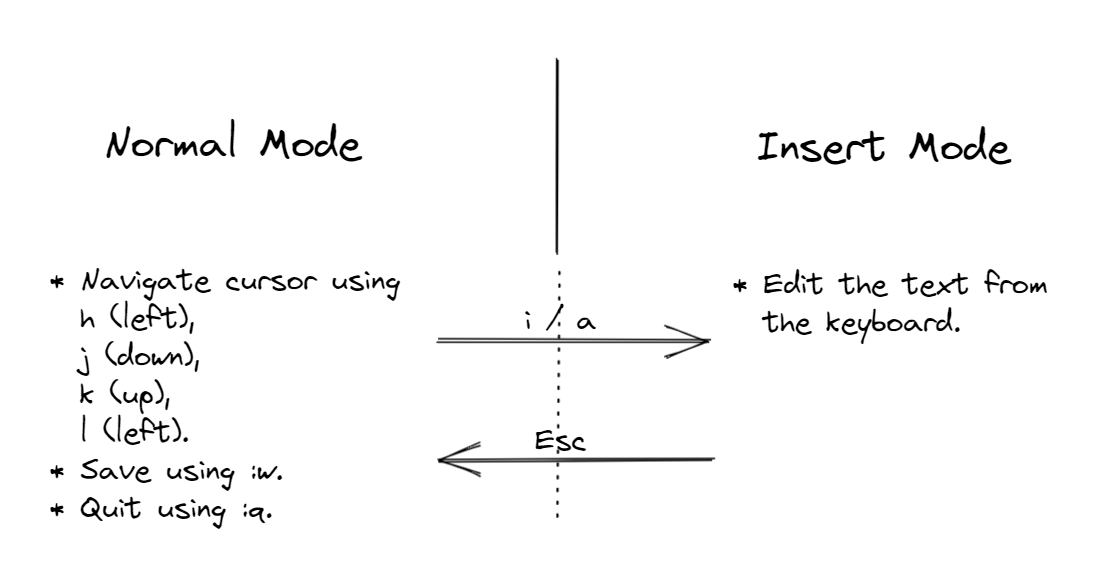
\includegraphics[width=250pt]{chapters/chapter3/figures/vimbasicmodeswitching.png}
\caption{Mode switching between normal mode and insert mode, and basic functions associated with the modes.} \label{ch3fig:vimbasicmodeswitching}
\end{figure}

\begin{figure}
\centering
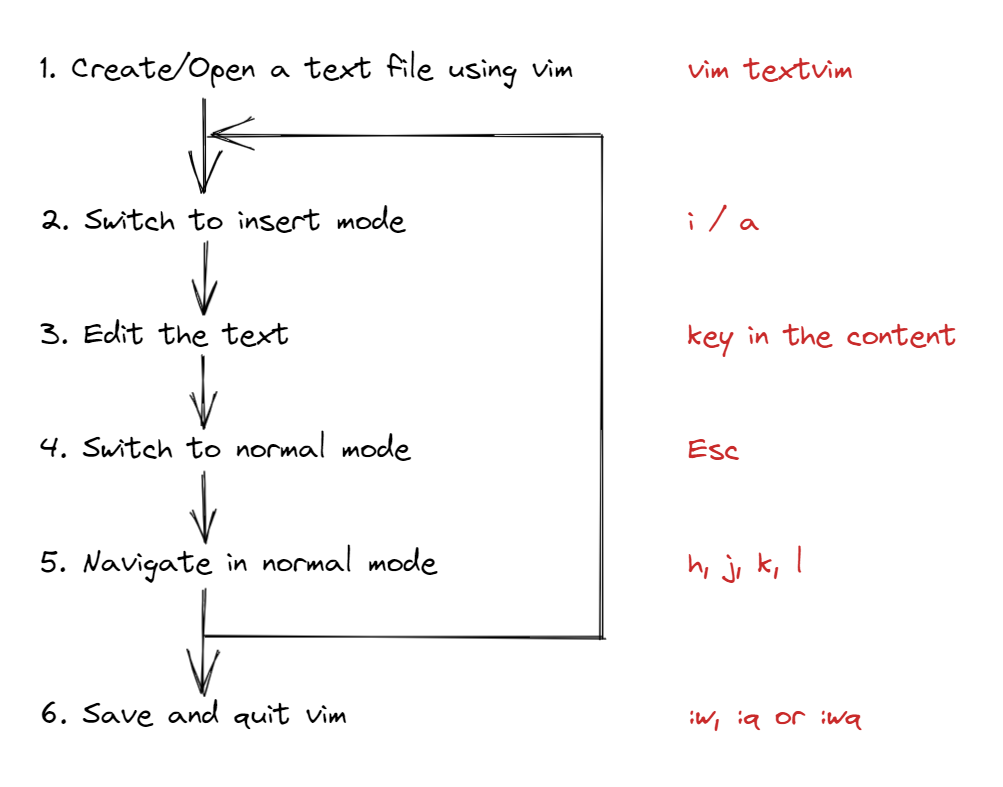
\includegraphics[width=250pt]{chapters/chapter3/figures/vimbasicoperationflowchart.png}
\caption{A flowchart for simple creating, editing and saving of a text file using \textit{Vim}.} \label{ch3fig:vimbasicoperationflowchart}
\end{figure}

There are other shortcuts to switch from normal mode to insert mode. Some of them are summarized in Table \ref{ch3tab:switchtoinsert}.

\begin{table}
  \centering \caption{Commonly used shortcuts to switch from normal mode to insert mode.}\label{ch3tab:switchtoinsert}
  \begin{tabularx}{\textwidth}{lX}
    \hline
    Operator & Description \\ \hline
    \verb|i| & Insert before the character at the cursor. \\ \hdashline
    \verb|I| & Insert at the beginning of the row at the cursor. \\ \hdashline
    \verb|a| & Insert after the character at the cursor. \\ \hdashline
    \verb|A| & Insert at the end of the row at the cursor. \\ \hdashline
    \verb|o| & Create a new row below the cursor and switch to insert mode. \\ \hdashline
    \verb|O| & Create a new row above the cursor and switch to insert mode. \\ 
    \hline
  \end{tabularx}
\end{table}

\subsection{Configure Customizable User Profile}

With the basic operations introduced in Section \ref{ch3subsec:vimgeneralintro}, we are able to create and edit a text file as we want to, just like using any other text editor. Though at this point the advantages of using \textit{Vim} over other text editors are not obvious yet, the \textit{Vim} editor is finally useful now.

Before introducing more advanced features of \textit{Vim} for more convenient user experience, we can now customize user profile to suit our individual habit. Notice that the customization is completely optional and personal. This section only introduces the ideas and basic methods of such customization, such as re-mapping keys and create user-defined shortcuts. Everything introduced here are merely examples and it is completely up to the user how to design and implement his own profile.

In Linux, navigate to home directory. Create the following path and file \verb|~/.vim/vimrc| or \verb|~/.vimrc|. Open the \textit{vimrc} file as a blank file using \textit{Vim}. The individual user profile can be customized here.

\vspace{0.1in}
\noindent \textbf{Mapping of Keys}
\vspace{0.1in}

It is desirable to re-map some keys to speed up editing. For example, people may want to map \verb|jj| to \verb|Esc| in insert mode for more convenient mode switching to normal mode (consequent ``jj'' is rarely used in English). Other people may feel like mapping \verb|j|, \verb|k|, \verb|i| to \verb|h|, \verb|j|, \verb|k| respectively in normal and visual modes, making the navigation more intuitive. In that case, a different key needs to be mapped for \verb|i| since it is an important key for switching to insert mode.

It is possible re-map certain key (or keys combination) in selected modes. The following configuration in \textit{vimrc} file re-maps the aforementioned keys.
\begin{verbatim}
inoremap jj <Esc>
noremap j h
noremap J H
noremap k j
noremap K J
noremap i k
noremap I K
noremap h i
noremap H I
\end{verbatim}
where \verb|inoremap| is used to map keys (combinations) in insert mode, and \verb|noremap| in normal and visual modes.

The upper case letter \verb|S| and lower case letter |s| in control mode are originally used to delete and substitute texts. They may be not so important in practice as there functions are overlapped by another shortcut key \verb|c|, which is powerful in replacing characters and is more frequently used. We can re-map \verb|S| for saving the text, and disable \verb|s| to prevent mis-touching. Similarly, upper case letter \verb|Q| is mapped to quit \textit{Vim}.
\begin{verbatim}
noremap s <nop>
map S :w<CR>
map Q :q<CR>
\end{verbatim}
where \verb|<nop>| stands for ``no operation'' and \verb|CR| stands for the ``enter'' key on the keyboard. The keyword \verb|map| differs from \verb|noremap| in the sense that \verb|map| is for recursive mapping.

\vspace{0.1in}
\noindent \textbf{Syntax Highlight, Color Scheme and Others}
\vspace{0.1in}

By default \textit{Vim} displays white color contents on black background. Use the following command in \textit{vimrc} to enable syntax highlighting or change color scheme. Use \verb|:colorscheme| in normal mode in \textit{Vim} to check for available color schemes.
\begin{verbatim}
syntax on
colorscheme default
\end{verbatim}

The following command displays the row index and cursor line (a underline at cursor position) of the text, which can become handy during the programming. Furthermore, it sets auto-wrap of text when a single row is longer than the displaying screen.
\begin{verbatim}
set number
set cursorline
set wrap
\end{verbatim}

The following command opens a ``menu'' when using cmdline mode, making it easier to key in commands.
\begin{verbatim}
set wildmenu
\end{verbatim}

Many users in the community have posted their recommended \textit{Vim} user profile configuration online, such as on \textit{GitHub}. For the convenience of the reader, in the rest of the notebook, we will assume that \textbf{no re-map of keys combinations or shortcuts} are implemented, when introducing the commands.

Notice that the configurations introduced in this section can also be activated with the \textit{Vim} already started. Simply type \verb|:| to switch from normal mode to cmdline mode, then key in the configuration. For example, \verb|:syntax on| to activate the syntax display.

\subsection{Commonly Used Operations in Normal Mode}

The operations, such as delete, cut, copy, paste, replace and search, are mostly done in normal mode through shortcut keys. For example, \verb|dd| delete (cut) the entire row at the cursor and \verb|p| paste the row to its new position. For beginners, remembering shortcut keys can be difficult. In such case, it is recommended for us to look for the consistent patterns of the different commands, instead of brute-force remembering the keys only.

Many \textit{Vim} shortcut keys in normal mode has the following structure, i.e. an operator command followed by a motion command, as shown below.
\begin{verbatim}
<operator><motion>
\end{verbatim}
The operator command tells \textit{Vim} what to do (say, copy), and the motion command tells the applicable range of the operation (say, the entire row, or the single word, or the single character, of the cursor position). Of course for some operator commands, they can be used alone without the motion command.

\vspace{0.1in}
\noindent \textbf{Delete/Cut, Change, Copy and Paste}
\vspace{0.1in}

We will use the most commonly used operator commands, delete/cut, change, copy (also known as ``yank'' in \textit{Vim}) and paste to demonstrate the above idea.

In this demonstration, we will be editing the following lines taken from Wikipedia under ``William Shakespeare''. In the text file, each sentence takes a new row as given by Figure \ref{ch3fig:vimdemo1}.

\begin{shortbox}
William Shakespeare (bapt. 26 April 1564 – 23 April 1616) was an English playwright, poet and actor, widely regarded as the greatest writer in the English language and the world's greatest dramatist.

He is often called England's national poet and the ``Bard of Avon'' (or simply ``the Bard'').
\end{shortbox}

\begin{figure}
\centering
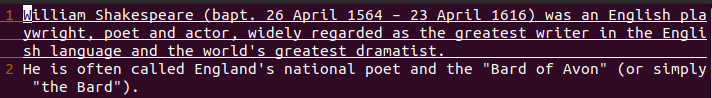
\includegraphics[width=250pt]{chapters/chapter3/figures/vimdemo1.png}
\caption{A piece of text of ``William Shakespeare'', for demonstration.} \label{ch3fig:vimdemo1}
\end{figure}

To quickly delete/cut a single character, use either \verb|x| or \verb|X|. Each time \verb|x| is input in normal mode, it deletes the current cursor selected character, and automatically select the next character in the text. Each time \verb|X| is input in normal mode, it keeps the current cursor selected character while deleting the previous character in front of the cursor. In this sense, \verb|x| and \verb|X| play like \verb|delete| and \verb|backspace| respectively in other text editors such as \textit{notepad++}.

Operators \verb|x| and \verb|X| do not require consequent motion command, as they simply delete/cut one character immediately each time they are pressed. What if you want to delete multiple characters from the cursor? You can press \verb|x| or \verb|X| multiple times, or alternatively you can ask \textit{Vim} to ``emulate'' doing that for you, as long as you tell \textit{Vim} what actions (key combinations) and how many times you want perform. For example, \verb|20x| is equivalent with physically pressing \verb|x| for 20 times. The same applies for other operators or motions commands. For example, \verb|10l| is equivalent of pressing \verb|l| for 10 times, making the navigation faster.

Operator \verb|d| does similar things as \verb|x| and \verb|X| but requiring a motion command, for more flexible usage. The motion shall tell \textit{Vim} what to delete/cut.

For example, \verb|dl| deletes to the right, i.e. deletes the current cursor selected character, and automatically select the next character. It is the same as if \verb|x| is pressed. Similarly, \verb|dh| deletes  to the left, just like \verb|X|. What if you want to delete 20 characters to the right? You can key in \verb|dl| for 20 times. Or alternatively, just like the case for \verb|x|, you can tell \textit{Vim} to do it by using \verb|20dl|. Or, you can change the motion, by using \verb|d20l|, where ``20l'' as a whole plays as the motion of ``to the right for 20 characters''. Or, you can do a combination by using things like \verb|5d4l|, since $20=5\times 4$. All of the above gives you the same result (they will be a difference in the clipboard if later you want to paste them).

Thanks to the ``operator-motion'' structure, \verb|d| can be used even more flexibly. For example, by using word-related motions, \verb|d| can delete/cut by words instead of by characters. Move the cursor to the beginning of a word, (for example, ``S'' in ``Shakespeare''), use \verb|dw| to delete the word. The word motion \verb|w| is similar with \verb|l|, except that \verb|l| directs to the next character, while \verb|w| directs to the beginning character of next word. Motion \verb|w| can also be used to navigate in the text. Similarly, \verb|b| directs to the beginning character of the current word (if the cursor is at the middle of the current word) or previous word (if the cursor is already at the beginning of the current word). Thus, \verb|db| can be used to delete word to the left. You can use something like \verb|d10b|, \verb|10db|, \verb|d20w|, \verb|5d4w| to delete multiple words at a time.

When in the middle of a word, \verb|dw| will delete the characters from the current cursor position till the beginning character of the next word. For example, if the cursor is currently at ``k'' in ``Shakespeare'', \verb|dw| will delete ``kespeare '' (notice that the space between ``Shakespeare'' and ``(bapt.'' will also be deleted). To delete from the beginning of the word instead of from the middle of the word, you can use \verb|b| first to navigate back to the beginning of the word. Alternatively, use ``inner-word'' motion \verb|iw| to indicate that you want to delete inner word. When the cursor is at ``k'' in ``Shakespeare'', use \verb|diw| to delete the entire word.

So far we have introduced the delete/cut operator \verb|d|, and character motion \verb|h| (left), \verb|l| (right), and also word motion \verb|b| (left), \verb|w| (right). There are similar motions for sentence \verb|(| (previous), \verb|)| (next) and paragraph \verb|{| (previous), \verb|}| (next). Finally, there is the inner-word motion \verb|iw| to indicate the current word of cursor, whichever the cursor is inside the word. Similarly, there are inner-sentence motion \verb|is| and inner-paragraph motion \verb|ip|. There are also inner-quotation motion \verb|i'|, \verb|i"|, \verb|i`| and inner-block motion \verb|i(|, \verb|i<|, \verb|i{|, and many more. For example, when cursor is at ``A'' of ``26 April 1564'', \verb|di(| will delete everything inside ``()'', i.e. deleting ``bapt. 26 April 1564 - 23 April 1616''.

To conclude, the operators and motions so far are listed in Tabs. \ref{ch3tab:deletecut} and \ref{ch3tab:motion}. Notice that motions \verb|aw|, \verb|as|, \verb|ap| are also given in the table. They are similar with their corresponding \verb|iw|, \verb|is|, \verb|ip| except that when deleting, the consequent blank space (for word and sentence) or blank row (for paragraph) will also be deleted. (Notice that \textit{Vim} marks the end of a sentence using ``.'', ``?'' or ``!'' followed by a space, tab or blank row, and the end of a paragraph by an empty row.)

\begin{table}
  \centering \caption{Commonly used operators related to delete/cut, change, copy and paste.}\label{ch3tab:deletecut}
  \begin{tabularx}{\textwidth}{lX}
    \hline
    Operator & Description \\ \hline
    \verb|x| & Delete/Cut the character at cursor. \\ \hdashline
    \verb|X| & Delete/Cut the character before cursor. \\ \hdashline
    \verb|dd| & Delete/Cut the entire row. \\ \hdashline
    \verb|d| & Delete/Cut selected text according to the motion command. \\ \hdashline
    \verb|cc| & Change the entire row. \\ \hdashline
    \verb|c| & Change selected text according to the motion command. \\ \hdashline
    \verb|yy| & Copy the entire row. \\ \hdashline
    \verb|y| & Copy selected text according to the motion command. \\ \hdashline
    \verb|p| & Paste clipboard to the cursor. \\
    \hline
  \end{tabularx}
\end{table}

\begin{table}
  \centering \caption{Commonly used motions.}\label{ch3tab:motion}
  \begin{tabularx}{\textwidth}{lX}
    \hline
    Motion & Description \\ \hline
    \verb|h|, \verb|l| & One character to the left or right. \\ \hdashline
    \verb|j|, \verb|k| & One row to the up or down. \\ \hdashline
    \verb|b|, \verb|w| & One word to the previous or next. \\ \hdashline
    \verb|(|, \verb|)| & One sentence to the previous or next. \\ \hdashline
    \lstinline{\{}, \lstinline{\}} & One paragraph to the previous or next. \\ \hdashline
    \verb|iw|, \verb|is|, \verb|ip| & inner-word, inner-sentence, inner-paragraph. \\ \hdashline
    \verb|aw|, \verb|as|, \verb|ap| & a word, a sentence, a paragraph (including the end blank). \\ \hdashline
    \verb|i'|, \verb|i"|, \verb|i`| & inner-quotation for different types of quotations. \\ \hdashline
    \verb|i(|, \verb|i<|, \verb|i[|, \lstinline{\}} & inner-block for different types of brackets. \\ \hdashline
    \verb|0| & Beginning of the row. \\ \hdashline
    \verb|$| & Ending of the row. \\ \hdashline
    \verb|gg| & Beginning of the text. \\ \hdashline
    \verb|G| & Beginning of the last row of the text. \\
    \hline
  \end{tabularx}
\end{table}

To change a piece of text, operator \verb|c| is used, followed by its associated motion to indicate the range of text to be changed. The same motions as given in Table \ref{ch3tab:motion} can be used. Effectively, operator $\verb|c|$ deletes/cut the text indicated by the motion first (just like operator \verb|d|), then switch to insert mode.

To copy a piece of text of clipboard, use \verb|y| (stands for ``yank'') followed by its associated motion to indicate the range of text. The motions also follow Table \ref{ch3tab:motion}.

To paste the text in the clipboard to the text at the cursor position, use \verb|p|. No motion is required.

In addition to the motions given in Table \ref{ch3tab:motion}, another commonly used method to navigate to a particular position if text is to ``find by character''. For example, consider the following row of text. The cursor is currently at letter ``A''.
\begin{verbatim}
ABCDEFG;HIJKLMN;OPQ;RST;UVW;XYZ
\end{verbatim}
In normal mode, using \verb|f| followed by a character will navigate the cursor to the nearest corresponding character that appears in the text. For example, \verb|fG| will move the cursor to letter ``G''. Similarly, \verb|f;| will move the cursor to the ``;'' between ``G'' and ``H''. Key in \verb|f;| again and the cursor will move to ``;'' between ``N'' and ``O''. From here key in \verb|2f:| and the cursor will go to ``;'' between ``T'' and ``U'', as it is equivalent to typing \verb|f;| twice.

\vspace{0.1in}
\noindent \textbf{Search in the Text}
\vspace{0.1in}

It is common that we want to search for a particular keywords or phrase, and highlight all of its appearances in the text. To make the searching result highlighted, add the following line to the user profile at \textit{vimrc}.
\begin{verbatim}
set hlsearch
exec "nohlsearch"
set incsearch
set ignorecase
\end{verbatim}
where \verb|hlsearch| highlights all matching results in the text, and \verb|incsearch| allows highlighting texts while keying in the word or phrase. Each time highlight search is enabled, \textit{Vim} will remember the keywords from the previous search and automatically hight them in the text, which can be confusing sometimes. The command \verb|exec "nohlsearch"| (\verb|exec| command in the user profile make \textit{Vim} execute that command when starting a new session) that comes after \verb|set hlsearch| resolves this issue by forcing \textit{Vim} to clear its memory. Finally, \verb|ignorecase| allows case insensitive while searching.

In normal mode, use \verb|/<keyword>| to search keywords or phrase. With the above setup, search for ``he'' using \verb|/he| will lead to the following result given in Fig.~\ref{ch3fig:vimdemo2}.
\begin{figure}
\centering
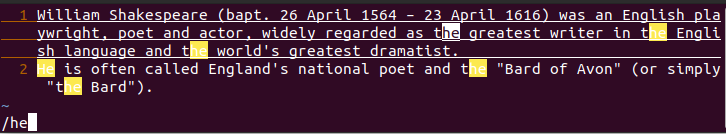
\includegraphics[width=250pt]{chapters/chapter3/figures/vimdemo2.png}
\caption{Search ``he'' in the piece of text of ``William Shakespeare''.} \label{ch3fig:vimdemo2}
\end{figure}
From Fig.~\ref{ch3fig:vimdemo2}, it can be seen that all appearances of ``he'' (case insensitive) is highlighted, and the cursor is automatically moved to the first appearance, i.e. ``he'' in ``and the world's greatest dramatist''. Click \verb|Enter| to quit searching. Now \verb|h|, \verb|j|, \verb|k| and \verb|l| can be used to navigate the cursor again, with the searching result maintain highlighted. Use \verb|n| and \verb|N| to navigate the cursor from the highlighted results. Notice that in this case, \verb|n| and \verb|N| can be used as motion together with delete/cut, change and copy as given in Table \ref{ch3tab:deletecut}.

To disable the existing searching highlight, either start searching a new keyword, or key in command \verb|:nohlsearch| in normal mode. For convenience, people may prefer to map it with a customized shortcut key as well, for example in \textit{vimrc} key in
\begin{verbatim}
noremap <Space> :nohlsearch<CR>
\end{verbatim}
so that \verb|Space| can be used to clear the search highlights.

\vspace{0.1in}
\noindent \textbf{Visual Mode}
\vspace{0.1in}

The use of a mouse makes selecting a block of text very intuitive. As your eyes move across the text, you can start selecting at any specific character or row by click-and-hold the mouse key, and end selecting at any specific character or row by simply letting it go. The selected text will be highlighted, as if the cursor expands from one character to the entire block of text. You can then perform operations such as delete or copy of the selected block of text.

When using \textit{Vim}, mouse is mostly useless. The visual mode of \textit{Vim} provides users a similar experience when selecting a block of text almost as if using a mouse.

It is possible to select multiple rows of text in visual mode, and then apply an operation all at rows simultaneously.



\subsection{Advanced Interface}


\subsection{Vim Accessories}



